\documentclass[landscape]{article}
\usepackage{tikz}
\usetikzlibrary{shapes,arrows,positioning,calc, arrows.meta}
\usepackage{geometry}


% Adjust the page layout with the geometry package
\geometry{left=1cm, right=1cm, top=1cm, bottom=1cm}


\begin{document}
\begin{figure}
    \centering
    \resizebox{\textwidth}{!}{

    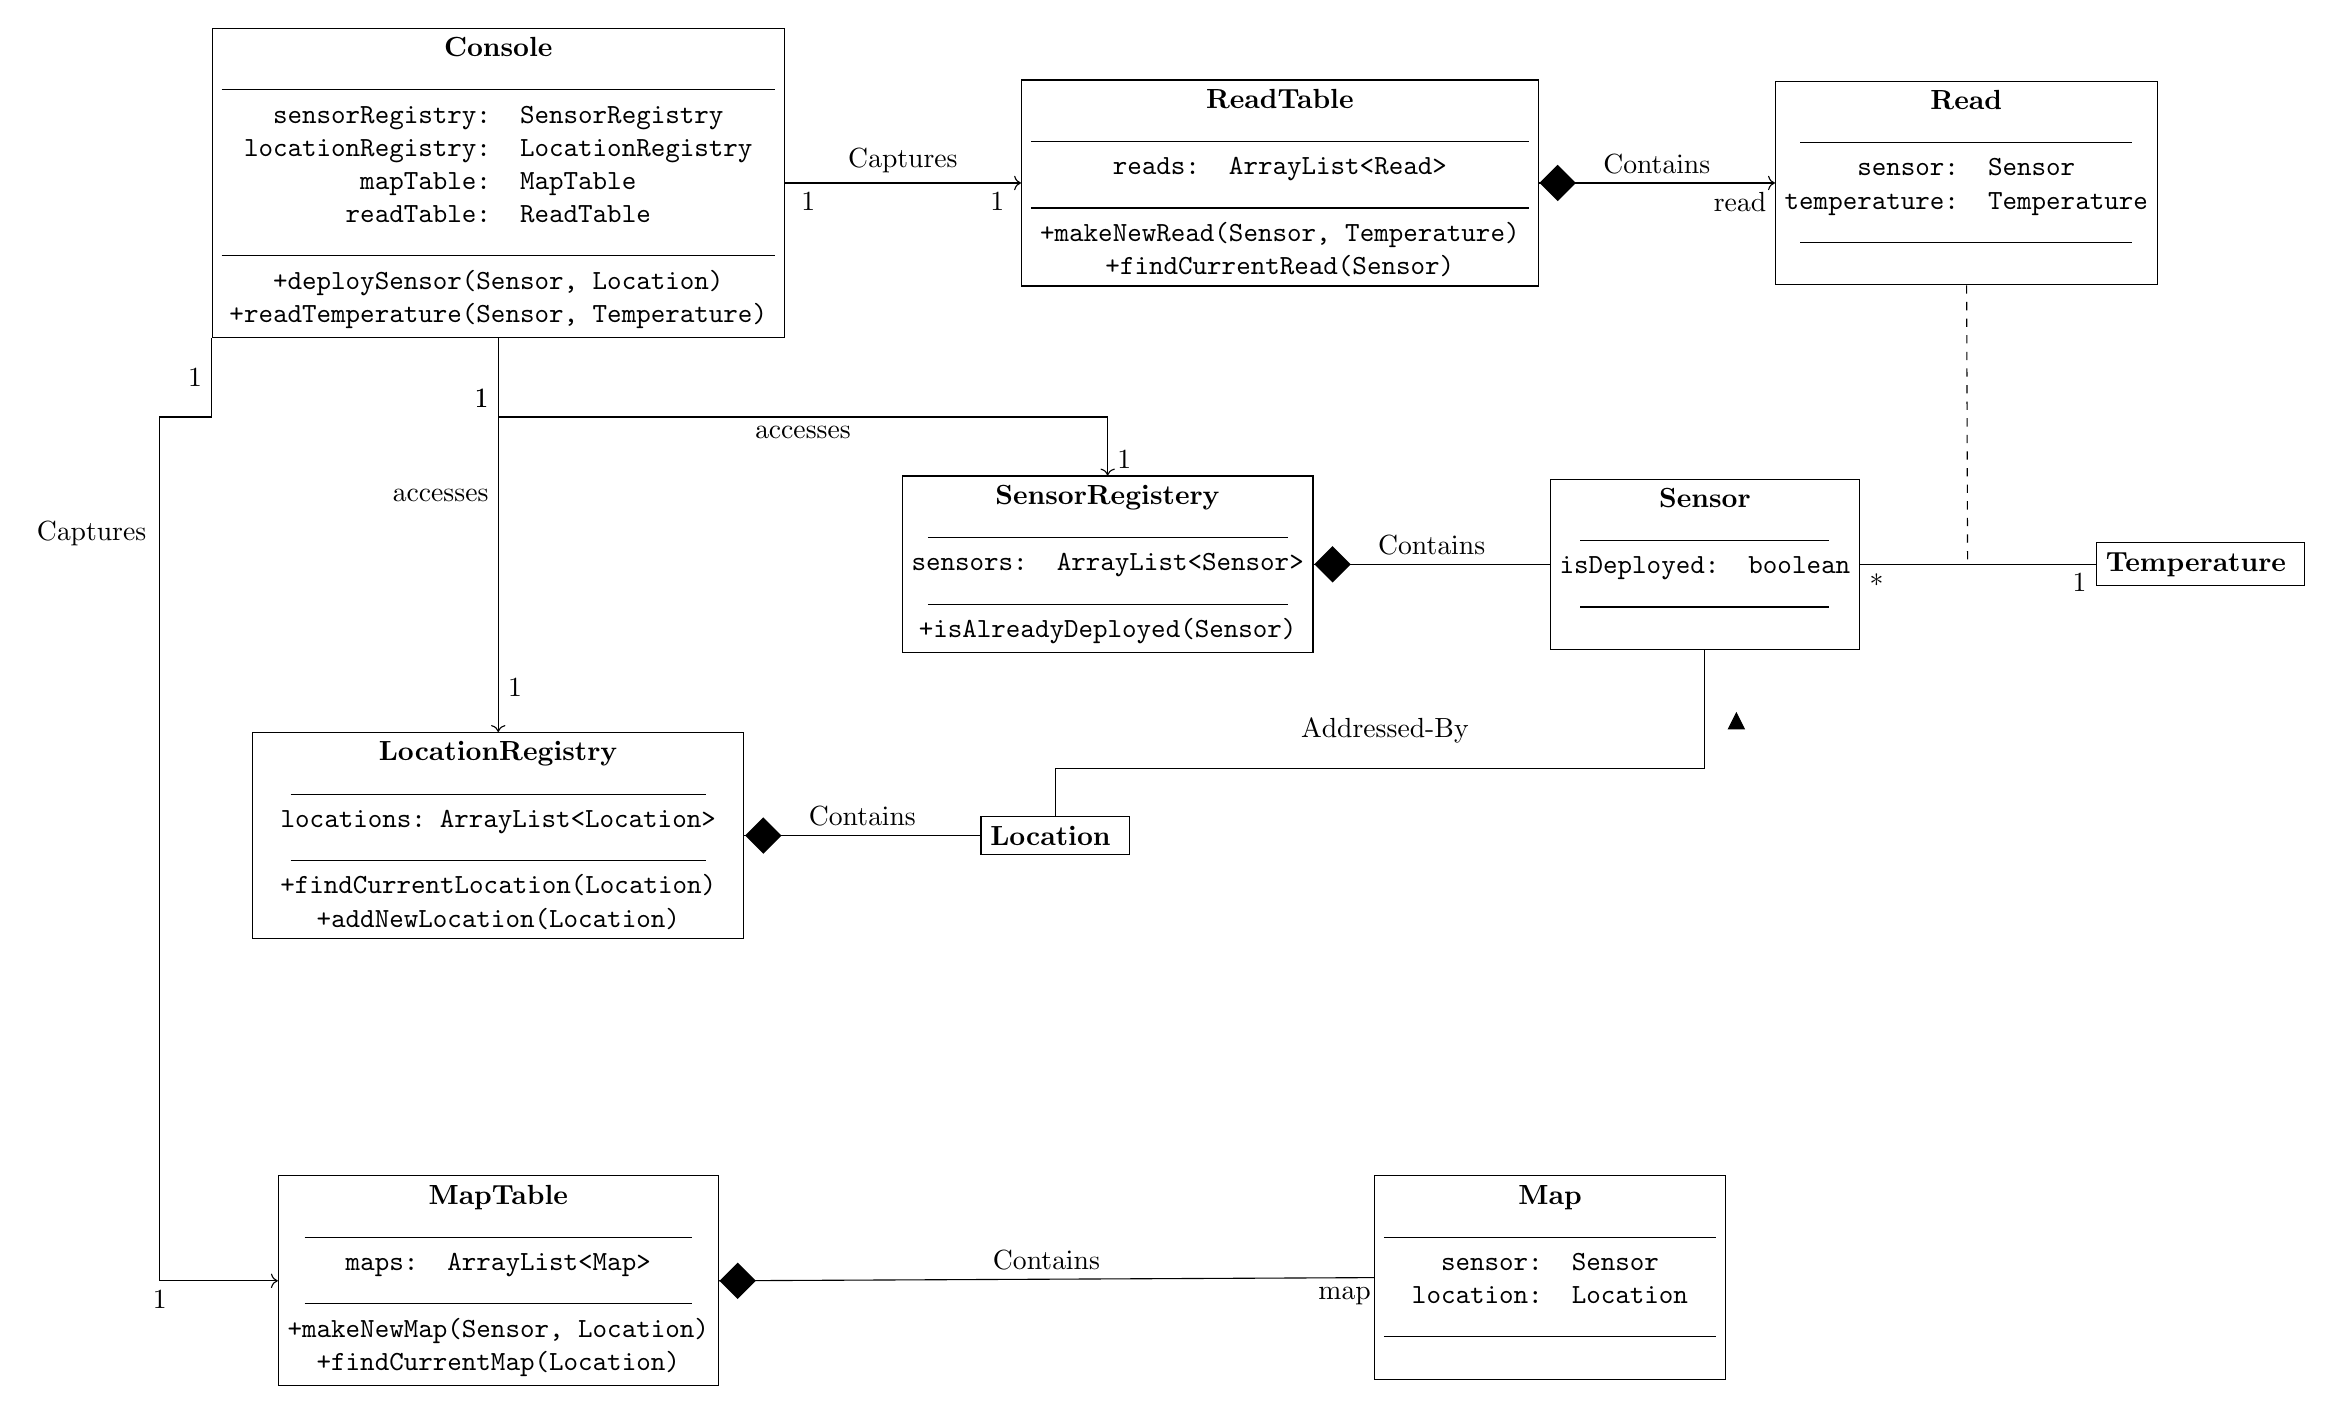
\begin{tikzpicture}
    
    	%-----Classes-----
        % Console Class
        \node [rectangle, draw, align=center] (console) {%
            \textbf{Console} \\
            \line(1,0){200} \\
            \texttt{sensorRegistry: SensorRegistry} \\
            \texttt{locationRegistry: LocationRegistry} \\
            \texttt{mapTable: MapTable} \\
            \texttt{readTable: ReadTable} \\
            \line(1,0){200} \\
            \texttt{+deploySensor(Sensor, Location)} \\
            \texttt{+readTemperature(Sensor, Temperature)}
        };
        
        % Location Registry Class
% Location Registry Class
\node [rectangle, draw, below=5cm of console, align=center, text width=6cm] (lreg) {%
    \textbf{LocationRegistry} \\
    \line(1,0){150} \\
    \texttt{locations: ArrayList<Location>} \\
    \line(1,0){150} \\
    \texttt{+findCurrentLocation(Location)} \\
    \texttt{+addNewLocation(Location)}
};

        % Read Table Class
        \node [rectangle, draw, right=3cm of console, align=center] (readt) {%
            \textbf{ReadTable} \\
            \line(1,0){180} \\
            \texttt{reads: ArrayList<Read>} \\
            \line(1,0){180} \\
            \texttt{+makeNewRead(Sensor, Temperature)} \\
            \texttt{+findCurrentRead(Sensor)}
        };
		
		 % Read Class
        \node [rectangle, draw, right=3cm of readt, align=center] (read) {%
            \textbf{Read} \\
            \line(1,0){120} \\
            \texttt{sensor: Sensor} \\
            \texttt{temperature: Temperature} \\
            \line(1,0){120} \\
        };
        
         % Sensor Registry Class
        \node [rectangle, draw, above right=1cm and 2cm of lreg, align=center] (sreg) {%
            \textbf{SensorRegistery}\\
            \line(1,0){130} \\
            \texttt{sensors: ArrayList<Sensor>} \\
            \line(1,0){130} \\
            \texttt{+isAlreadyDeployed(Sensor)}
        }; 
        
        % Sensor Class
        \node [rectangle, draw, right=3cm of sreg, align=center] (sensor) {%
            \textbf{Sensor} \\
            \line(1,0){90} \\
            \texttt{isDeployed: boolean} \\
            \line(1,0){90} \\
        };
       
       % Temperature Class
        \node [rectangle, draw, right=3cm of sensor, align=center] (temp) {%
            \textbf{Temperature} 
        };
        
        % Location Class
        \node [rectangle, draw, right=3cm of lreg, align=center] (loc) {%
            \textbf{Location} 
        };
        
        % Location Map Class
        %\node [rectangle, draw, below=2cm of loc, align=center] (locmap) {%
            %\textbf{LocationMap} 
        %};
        
        % Map Table Class
        \node [rectangle, draw, below=3cm of lreg, align=center] (mapt) {%
            \textbf{MapTable}  \\
            \line(1,0){140} \\
            \texttt{maps: ArrayList<Map>} \\
            \line(1,0){140} \\
            \texttt{+makeNewMap(Sensor, Location)} \\
            \texttt{+findCurrentMap(Location)}
        };
        
         % Map Class
        \node [rectangle, draw, below right=3cm and 8cm of lreg, align=center] (map) {%
            \textbf{Map}  \\
            \line(1,0){120} \\
            \texttt{sensor: Sensor} \\
            \texttt{location: Location} \\
            \line(1,0){120} \\
        };
        
        
\draw[->] (console) -- (readt) node[midway, above] {Captures} node[pos=0.9, below] {1} node[pos=0.1, below] {1};

        
        \node[diamond, fill=black, anchor=west, minimum size=10pt] at (readt.east) {};
\draw[->] (readt.east) -- (read.west) node[midway, above] {Contains} node[pos=0.7, below right] {read};

\draw[-] (sensor) -- (temp) node[midway, above] {} node[pos=0, below right] {*} node[pos=1, below left] {1};

\draw[dashed] (read) -- ($(sensor)!0.53!(temp)$) node[midway, above] {};

        \node[diamond, fill=black, anchor=west, minimum size=10pt] at (sreg.east) {};
\draw[-] (sreg.east) -- (sensor.west) node[midway, above]{Contains};



\draw[->] (console.south) -- ++(0,-1) -| (sreg.north)node[pos=0.25, below] {accesses} node[pos=0.0, above left] {1} node[pos=0.7, below right] {1};


% Arrow from console to location registry
\draw[->] (console.south) -- ++(0,-1) -| (lreg.north) node[pos=0.6, below left] {accesses} node[pos=0.0, above left] {1} node[pos=0.9, below right] {1};





% Arrow from the bottom left of Console to the top right of MapTable
% Arrow from Console to MapTable with 90-degree turns around LocationRegistry
\draw[->] (console.south west) -- ++(0,-1)node[pos=1.5, below left=1cm] {Captures} node[midway, left] {1} -| ([xshift=-1.5cm]mapt.west) node[pos=1, below] {1} -- (mapt.west);


        \node[diamond, fill=black, anchor=west, minimum size=10pt] at (lreg.east) {};
\draw[-] (lreg.east) -- (loc.west) node[midway, above]{Contains};

        \node[diamond, fill=black, anchor=west, minimum size=10pt] at (mapt.east) {};
\draw[-] (mapt.east) -- (map.west) node[midway, above]{Contains} node[pos=0.9, below right] {map};

\draw[-] (sensor.south) -- ++(0,-1.5cm) -| (loc.north) node[midway, above right=0.2cm and 3cm] {Addressed-By};

        \draw[black, fill=black] (sensor.south) ++(0.3,-1) -- ++(0.2,0) -- ++(-0.1,0.2) -- cycle;

        
    \end{tikzpicture}
    }
    \caption{UML Class Diagram for Sensor System}
\end{figure}
\end{document}
